\documentclass[12pt,a4paper,bibliography=totocnumbered,listof=totocnumbered]{scrartcl}
\usepackage[ngerman]{babel}
\usepackage[utf8]{inputenc}
\usepackage[T1]{fontenc}
\usepackage{lmodern}
\usepackage{amsmath}
\usepackage{amsfonts}
\usepackage{amssymb}
\usepackage{graphicx}
\usepackage{fancyhdr}
\usepackage{tabularx}
\usepackage{geometry}
\usepackage{setspace}
\usepackage[right]{eurosym}
\usepackage{acronym}
\usepackage{subfig}
\usepackage{floatflt}
\usepackage[usenames,dvipsnames]{color}
\usepackage{colortbl}
\usepackage{paralist}
\usepackage{array}
\usepackage{titlesec}
\usepackage{parskip}
\usepackage[right]{eurosym}
\usepackage[subfigure,titles]{tocloft}
\usepackage[pdfpagelabels=true]{hyperref}
\usepackage[singlelinecheck=false]{caption}
\usepackage{times}
\usepackage{rotating}
\usepackage{pdflscape}
\usepackage{pdfpages}
\usepackage{titlesec,blindtext}
\usepackage[style=authoryear,
    sorting=nyt,
    maxnames=19,
    firstinits,
    block=space]{biblatex}
\DeclareNameAlias{sortname}{last-first}
\DeclareNameAlias{default}{last-first}
\defbibheading{bibintoc}[\bibname]{%
               \chapter*{#1}%
               \markboth{#1}{#1}}
%\renewcommand{\sectionmark}[1]{\markright{#1}}
% Doppelpunkt nach Jahr
\renewcommand{\labelnamepunct}{\addcolon\space}
% Kapitälchen
\renewcommand*{\mkbibnamelast}[1]{\textsc{#1}}
% new URI font
\appto{\biburlsetup}{\renewcommand*{\UrlFont}{\normalfont}}
%Remove "and" before last name. However, this also removes "and" in a textcite...
\renewcommand*{\finalnamedelim}{\addsemicolon\space}
\DeclareFieldFormat[inbook,thesis]{title}{#1\addperiod} % italic title with period
\renewbibmacro*{volume+number+eid}{%
  \printfield{volume}%
%  \setunit*{\adddot}% DELETED
  \setunit*{\addnbspace}% NEW (optional); there's also \addnbthinspace
  \printfield{number}%
  \setunit{\addcomma\space}%
  \printfield{eid}}
\DeclareFieldFormat[article]{number}{\mkbibparens{#1}}

               
               


%\usepackage[babel,german=guillemets]{csquotes}
\addbibresource{bibo.bib}


\usepackage{listings}
\lstset{basicstyle=\footnotesize, captionpos=b, breaklines=true, showstringspaces=false, tabsize=2, frame=lines, numbers=left, numberstyle=\tiny, xleftmargin=2em, framexleftmargin=2em}
\makeatletter
\def\l@lstlisting#1#2{\@dottedtocline{1}{0em}{1em}{\hspace{1,5em} Lst. #1}{#2}}
\makeatother

\geometry{a4paper, top=25mm, left=25mm, right=30mm, bottom=25mm, headsep=12mm, footskip=12mm}

\hypersetup{unicode=false, pdftoolbar=true, pdfmenubar=true, pdffitwindow=false, pdfstartview={FitH},
	pdftitle={Abschlussarbeit},
	pdfauthor={Lisa Düpre},
	pdfsubject={Abschlussarbeit},
	pdfcreator={\LaTeX\ with package \flqq hyperref\frqq},
	pdfproducer={pdfTeX \the\pdftexversion.\pdftexrevision},
	pdfkeywords={Abschlussarbeit},
	pdfnewwindow=true,
	colorlinks=true,linkcolor=black,citecolor=black,filecolor=magenta,urlcolor=black}
\pdfinfo{/CreationDate (D:20110620133321)}

% Paragraph soll das neue subsubsubsection werden
\makeatletter
\renewcommand\paragraph{\@startsection{paragraph}{4}{\z@}%
            {-2.5ex\@plus -1ex \@minus -.25ex}%
            {0.1px}%
            {\normalfont\normalsize}
}
\makeatother
\titlespacing{\paragraph}{0mm}{10pt}{1pt} % funktioniert bestens


\setcounter{secnumdepth}{4} % how many sectioning levels to assign numbers to
\setcounter{tocdepth}{4}    % how many sectioning levels to show in ToC


\titleformat*{\section}{\large\bfseries\sffamily}
\titleformat*{\subsection}{\normalfont\bfseries\sffamily}
\titleformat*{\subsubsection}{\normalfont\normalsize}

% word mäßiger Zeilenabstand 
\usepackage{setspace}
\newcommand{\MSonehalfspacing}{
    \setstretch {1.433}
}

\begin{document}

\titlespacing{\section}{0pt}{12pt plus 4pt minus 2pt}{-6pt plus 2pt minus 2pt}

% Kopf- und Fusszeile
\renewcommand{\sectionmark}[1]{\markright{#1}}
\renewcommand{\leftmark}{\rightmark}
\pagestyle{fancy}
\lhead{}
\chead{}
\rhead{\thesection\space\contentsname}
%\lfoot{Möglichkeiten und Grenzen \newline computergestützter Ernährungserhebungsmethoden}
\cfoot{}
\rfoot{\ \linebreak Seite \thepage}
\renewcommand{\headrulewidth}{0.4pt}
\renewcommand{\footrulewidth}{0.4pt}

% Vorspann
\renewcommand{\thesection}{\Roman{section}}
\renewcommand{\theHsection}{\Roman{section}}
\pagenumbering{Roman}

% ----------------------------------------------------------------------------------------------------------
% Titelseite
% ----------------------------------------------------------------------------------------------------------
\thispagestyle{empty}
\begin{center}
	%
\includegraphics[scale=.2]{Bilder/640px-Uni_Bonn.png}\\
	%\vspace*{2cm}
          \normalsize
	\textbf{RHEINISCHE FRIEDRICH – WILHELMS – UNIVERSITÄT BONN}\\
	\vspace*{0.5cm}
	\normalsize
	\textbf{Landwirtschaftliche Fakultät}\\
	\vspace*{2cm}
	\Large
	\textbf{BACHELORARBEIT}\\
	\vspace*{0.4cm}
	\large
	im Rahmen des Bachelorstudiengangs\\
           \vspace*{0.4cm}
           \textbf{Ernährungs- und Lebensmittelwissenschaften}\\
           \vspace*{0.4cm}
	\large
           zur Erlangung des Grades\\
           \vspace*{0.4cm}
           \textbf{"Bachelor of Science"}\\
	\vspace*{3cm}
           \Large
	\textbf{Möglichkeiten und Grenzen von computergestützten Ernährungserhebungsmethoden}\\
	
    \vspace*{3cm}
    \normalsize {vorgelegt von:\\[0.8cm]}
	\normalsize
    Lisa Düpre \\[0.2cm]
         2477851\\[1cm]
         vorgelegt am  27.10.2014 
         \vfill
	\newcolumntype{x}[1]{>{\raggedleft\arraybackslash\hspace{0pt}}p{#1}}
	\begin{tabular}{x{6cm}p{7.5cm}}
		\rule{0mm}{5ex}\textbf{1. Prüfende/Prüfer:} & Prof. Dr. Monika Hartmann \\ 
                     \rule{0mm}{5ex}\textbf{2. Prüfende/Prüfer:} & Dipl.oecotroph. Julia Haß \\ 
		
	\end{tabular} 
\end{center}
\pagebreak



% ----------------------------------------------------------------------------------------------------------
% Verzeichnisse
% ----------------------------------------------------------------------------------------------------------
% TODO Typ vor Nummer
\renewcommand{\cfttabpresnum}{Tab. }
\renewcommand{\cftfigpresnum}{Abb. }
\settowidth{\cfttabnumwidth}{Abb. 10\quad}
\settowidth{\cftfignumwidth}{Abb. 10\quad}

\titlespacing{\section}{0pt}{12pt plus 4pt minus 2pt}{2pt plus 2pt minus 2pt}
\singlespacing
\rhead{INHALTSVERZEICHNIS}
\renewcommand{\contentsname}{Inhaltsverzeichnis}
\phantomsection
%\addcontentsline{toc}{section}{\texorpdfstring{I \hspace{0.35em}Inhaltsverzeichnis}{Inhaltsverzeichnis}}
%\addtocounter{section}{1}
\tableofcontents
\pagebreak
\rhead{VERZEICHNISSE}
\listoffigures


% bei Bedarf eines Tabellenverzeichnis wieder reinnehmen
\listoftables
%\pagebreak
%\renewcommand{\lstlistlistingname}{Listing-Verzeichnis}
%{\labelsep2cm\lstlistoflistings}
\pagebreak

% ----------------------------------------------------------------------------------------------------------
% Abkürzungen
% ----------------------------------------------------------------------------------------------------------

\section{Abkürzungsverzeichnis}

\begin{acronym}[LISAJERO] 
%\setlength{\itemsep}{0.3\parsep}

\acro{AMPM} {Automated Multiple Pass Method}
\acro{ASA24}{Automated Self-Administered 24-hour Recall}
\acro{DLW} {Doubly Labeled Water}
\acro{DPFM} {Digital Photography of Foods Method} 
\acro{EA} {Energieaufnahme}
\acro{ENA} {Energie- und Nährstoffaufnahme} 
\acro{MBK}{Mahlzeitenbasierte Kurzliste}
\acro{mdFR} {Mobile Device Food Record} 
\acro{MMM} 	{My Meal Mate}
\acro{NHANES} {National Health and Nutrition Examination Survey}
\acro{PDA}{Personal Digital Assistants}
\acro{RFPM} {Remote Food Photography Method} 
\acro{SMS}{Short Message Service}
\acro{WHO} {World Health Organization}
\end{acronym}

\newpage

% ----------------------------------------------------------------------------------------------------------
% Inhalt
% ----------------------------------------------------------------------------------------------------------
% Abstände Überschrift
\titlespacing{\section}{0pt}{12pt plus 4pt minus 2pt}{-6pt plus 2pt minus 2pt}
\titlespacing{\subsection}{0pt}{12pt plus 4pt minus 2pt}{-6pt plus 2pt minus 2pt}
\titlespacing{\subsubsection}{0pt}{12pt plus 4pt minus 2pt}{-6pt plus 2pt minus 2pt}

% Kopfzeile
\renewcommand{\sectionmark}[1]{\markright{#1}}
\renewcommand{\subsectionmark}[1]{}
\renewcommand{\subsubsectionmark}[1]{}
\lhead{Kapitel \thesection}
\rhead{\rightmark}

%\onehalfspacing
%\linespread{1.4}
\MSonehalfspacing
\selectfont

\renewcommand{\thesection}{\arabic{section}}
\renewcommand{\theHsection}{\arabic{section}}
\setcounter{section}{0}
\pagenumbering{arabic}
\setcounter{page}{1}

% ---------------------------- Hier kannst Du die Kapitel einfügen ---------------------

% ----------------------------------------------------------------------------------------------------------
% Einleitung
% ----------------------------------------------------------------------------------------------------------
\section{Einleitung}

\subsection{Problemstellung}
Die Erhebung der menschlichen  Ernährung ist schon lange ein wichtiges Werkzeug, um Informationen über das Essverhalten bestimmter Bevölkerungsgruppen zu erhalten und Zusammenhänge zwischen Ernährung und Gesundheit aufzudecken (Müller, 2007).
Um diese Ziele zu erreichen, muss das Ernährungsverhalten einer Person möglichst genau erfasst werden. Untersuchungen des Verzehrverhaltens bieten wertvolle Erkenntnisse, um Interventionsprogramme zur Prävention von chronischen Krankheiten zu gestalten (Six et al. 2010). Nach  Angaben der World Health Organization (WHO) hat sich weltweit seit 1980 die Zahl der Übergewichtigen verdoppelt. Im Jahr 2008 waren mehr als 1,4 Milliarden Erwachsene übergewichtig (davon über 200 Millionen Männer und fast 300 Millionen Frauen) (vgl. WHO). Die Folgen von Fehlernährung sind schwere gesundheitliche Probleme wie Diabetes, Schlaganfall und Herzerkrankungen sowie hohe Kosten im Gesundheitswesen (Wirth und Hauner, 2008). Die auf die anhaltende Zunahme von Übergewicht und Adipositas zurückzuführenden Ausgaben führen zu einem erhöhten Interesse, praktische und neue Technologien zur Prävention der Adipositas zu erforschen (Ershow et al., 2004). Um das Essverhalten zu registrieren, wurden verschiedene Methoden entwickelt, die sich je nach Ziel und Umfang der Erfassung unterscheiden. Aus den erhobenen Informationen werden mittels verschiedener Datenbanken Nährstoff- und Energiezufuhr berechnet. Anhand der Ergebnisse können Rückschlüsse auf den Ernährungsstatus eines Menschen geschlossen werden. Jedoch sind Durchführung und Auswertung der meisten traditionellen Methoden wie dem Verzehrsprotokoll sehr zeitaufwendig und setzen eine hohe Folgebereitschaft der Nutzer voraus. Zudem sind sie oft kostenintensiv und es kommt häufig zu Problemen und Fehlern, vor allem durch falsches Schätzen der Portionsgrößen, Underreporting oder mangelndem Erinnerungsvermögen der Probanden. Somit entstehen ungenaue Ergebnisse, die zu falschen Beurteilungen und Rückschlüssen führen können (Schneider und Heseker, 2006).


Um die Ernährungserhebung zuverlässiger zu gestalten und besonders vor dem Hintergrund der stetig wachsenden Zahl ernährungsbedingter Krankheiten, ist es wichtig, Ernährungserhebungsmethoden zu entwickeln, die 
\begin{itemize}
\item valide,
\item prospektiv,
\item für den Alltag geeignet,
\item einfach und schnell in der Handhabung,
\item kostengünstig,
\item möglichst fehlerfrei sind.
\end{itemize}

Weiterhin sollen sie vor allem
\begin{itemize}
\item Portionsgrößen präzise berechnen
\item Underreporting vermeiden (Kovatsch, 2014).
\end{itemize}

Mit dem technologischen Fortschritt in vielen Bereichen des Gesundheitswesens, wurden in den letzten Jahren Methoden zur Ernährungserhebung entwickelt, die auf Computerprogramme zurückgreifen. Diese sollen die Erhebung effizienter gestalten. 


\subsection{Zielsetzung}

Durch die Einführung von computergestützten Methoden, stellt sich die Frage, ob und wie gut die bisher entwickelten Verfahren die in Kapitel 1.1 genannten Kriterien erfüllen. Zudem ergeben sich mit den neuen Methoden auch neue Probleme, wie zum Beispiel die Tatsache, dass sie für den Umgang mit Computern oder anderen elektronischen Geräten  ein Grundmaß an Erfahrung erfordern (Kirkpatrick et al.,2014). Welche bisher bestehenden Probleme gelöst werden und welche Schwierigkeiten mit der Einführung entstehen, wird in dieser Bachelorarbeit beschrieben. Weiterhin wird aufgezeigt, für welche Zielgruppen die verschiedenen Methoden geeignet sind.
Somit werden die Möglichkeiten und Grenzen von computergestützten Ernährungserhebungsmethoden aufgezeigt und die Anwendbarkeit dieser Methoden beurteilt. 

\subsection{Vorgehensweise}

Die Arbeit ist in folgende fünf Hauptkapitel gegliedert. Im \textbf{ersten Kapitel} findet eine Heranführung an das Thema dieser wissenschaftlichen Arbeit statt, indem die Problemstellung und die Zielsetzung genau definiert werden. Das \textbf{zweite Kapitel} beleuchtet zunächst allgemein Ziele von Ernährungserhebungen. Es folgt ein Überblick über die traditionellen Methoden, die in der Erfassung der Ernährung angewandt werden. Dabei werden die gängigsten direkten Methoden beschrieben. Daraufhin werden aktuelle, computergestützte Methoden vorgestellt. Es wird ein Überblick über die bisher entwickelten Methoden gegeben und sechs Methoden näher beschrieben. Im Anschluss werden im \textbf{dritten Kapitel} ausgewählte Studien und deren Ergebnisse beschrieben, welche die aufgeführten Erhebungsmethoden prüfen.  Im \textbf{vierten Kapitel} werden die Studienergebnisse diskutiert. Aus diesem Kapitel gehen die Vor- und Nachteile der einzelnen Methoden hervor. Schließlich bildet das \textbf{fünfte Kapitel} den inhaltlichen Abschluss der Bachelorarbeit. Es beinhaltet in Form einer Empfehlung ein Fazit und einen Ausblick auf die neusten Methoden.



\pagebreak
% ----------------------------------------------------------------------------------------------------------
% Kapitel
% ----------------------------------------------------------------------------------------------------------
\newpage
\section{Übersicht über Ernährungserhebungsmethoden}

Ernährungserhebungsmethoden lassen sich in indirekte und direkte Methoden einteilen. Die indirekte Erfassung der Ernährung basiert auf der Sammlung statistischer Daten von Populationen oder Teilpopulationen, wie z.B. Agrarstatistiken, Einkommens- und Verbrauchsstatistiken. So können u.a. Ernährungssituationen verschiedener Länder gegenübergestellt werden. Direkte Methoden erfassen das individuelle Ernährungsverhalten einzelner Menschen. Sie werden nochmals in prospektive und retrospektive Methoden unterteilt (Müller, 2007). 

\subsection{Ziele von Ernährungserhebung}

Ernährungserhebungen werden durchgeführt, um den Lebensmittelverzehr einzelner oder mehrerer Personen zu erfassen. Wichtig ist die Erhebung im Gebiet der Ernährungsberatung, der Diagnose von Erkrankungen, Allergien und Unverträglichkeiten. Durch eine valide Erfassung und Auswertung des Lebensmittelverzehrs im Rahmen wissenschaftlicher Studien können außerdem Zusammenhänge zwischen der Ernährung und verschiedener ernährungsbedingter Erkrankungen ermittelt werden. Fehlernährung gilt neben erhöhtem Blutdruck, hohen Blutfettwerten und Übergewicht zu den bedeutendsten Risikofaktoren chronischer Erkrankungen. Genaue Auskünfte über das Ernährungsverhalten sind daher ein wichtiger Faktor für Behandlung und Prävention solcher Krankheiten (Hurrelmann, 2004).

\subsection{Traditionelle direkte Ernährungserhebungsmethoden}

Direkte Methoden ermitteln den Verzehr von Lebensmitteln individuell und betreffen so unmittelbar die Ernährung einzelner Personen. Sie lassen sich in zwei verschiedene Kategorien unterteilen: retrospektive und prospektive Methoden. Retrospektive Methoden sind Interviewmethoden und beziehen sich auf das zurückliegende Ernährungsverhalten einer Person. Prospektive Methoden dagegen sind Protokollmethoden und erfassen den gegenwärtigen Verzehr (Sichert et al., 1984).

%TODO:
%Abb.1 Gliederung der traditionellen Ernährungserhebungsmethoden
\begin{figure}[!h]
	\centering
		
	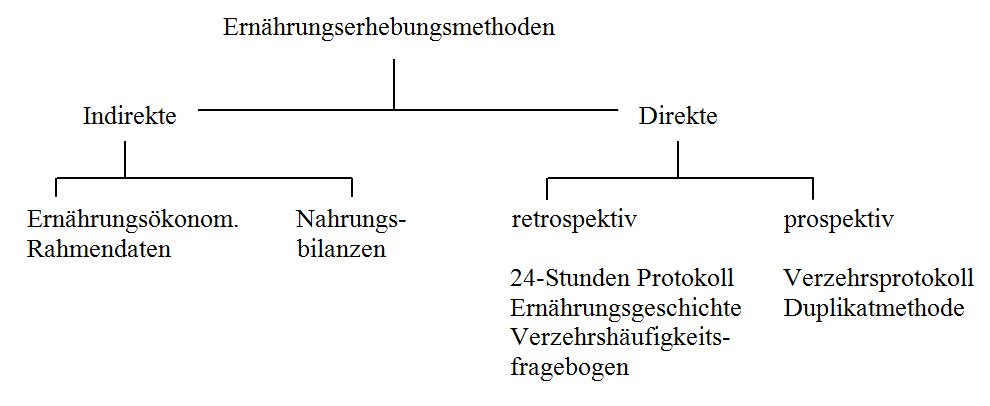
\includegraphics[width=0.9\textwidth]{Bilder/Abb1.png}

	\caption[Gliederung der traditionellen Ernährungserhebungsmethoden]{Gliederung der traditionellen Ernährungserhebungsmethoden.\\ Quelle: Modifiziert nach Sichert et al., 1984}
	\label{bild2}
\end{figure}

\subsubsection{Retrospektive Methoden}

Retrospektive Methoden beziehen sich auf den vergangenen Verzehr. Je nach Methode bezieht sich die Erhebung auf einen kurzen Zeitraum (24-Stunden Erinnerungsprotokoll) oder längere Zeiträume von bis zu mehreren Monaten (Ernährungsgeschichte). Es gilt, dass der Nahrungsverzehr einer Person nach Art und Menge für den festgelegten Zeitraum so genau wie möglich erfasst wird (Müller, 2007).

\paragraph{24-Stunden Erinnerungsprotokoll}

Das 24-Stunden Erinnerungsprotokoll (24-hour Recall) besteht aus einer Auflistung der Nahrungsaufnahme des Vortages bzw. der vergangenen 24 Stunden. Der Befragte wird gebeten, sich an alle Nahrungsmittel inklusive Mengen zu erinnern, die er in den letzten 24 Stunden aufgenommen hat. Zu Beginn erfragt ein geschulter Interviewer, welche Lebensmittel in welchen Mengen vom Teilnehmer in den letzten 24 Stunden verzehrt wurden. Daraufhin werden die verzehrten Lebensmittel nach Art und Menge identifiziert. Es folgt eine Umrechnung der Mengenschätzungen in Gewichtseinheiten und schließlich die Berechnung der Inhaltsstoffe mittels Nährwerttabellen bzw. Lebensmitteldatenbanken. Die Mengenangaben werden in haushaltsüblichen Größen (z.B. Tasse, Löffel, Stück) angegeben und erfasst. Um die Angaben von Portionsgrößen zu erleichtern, können Hilfsmittel wie Bilder oder Schablonen herangezogen werden (Sichert et al. 1984). In Tabelle 1 sind Vor- und Nachteile des 24-Stunden Protokolls aufgeführt.


% TODO: TABELLEN AN RICHTIGE STELLE SETZEN 

%Tab.1: Vor- und Nachteile beim 24-Stunden Erinnerungsprotokoll
%----------------------------------------------- 1. Tabelle: 24-Stunden Erinnerungsprotokoll -----------------------------------------------

\begin{table}[!h]
\begin{flushleft}
\caption{Vor- und Nachteile beim 24-Stunden Erinnerungsprotokoll}
\end{flushleft}
\begin{tabular}{p{7cm} p{7cm}}
Vorteile & Nachteile \\
\hline

\begin{itemize}
\item geringer zeitlicher, personeller und finanzieller Aufwand
\item gut einsetzbar und leichte Durchführung
\item große Stichprobenzahl möglich
\item keine Beeinflussung des Ernährungsverhaltens
\item Befragungsaufwand für die Teilnehmer gering und daher hohe Compliance
\item kurzer Zeitraum zwischen Verzehr und Befragung
\item genaue Angaben zu Häufigkeiten und Mengen der Lebensmittel möglich
\item nichtreaktive Erhebungsmethode

\end{itemize}

&

\begin{itemize}
\item selten verzehrte Lebensmittel werden eventuell nicht erfasst
\item nur die Erfassung des aktuellen Verzehrs ist möglich, nicht des üblichen
\item Ergebnisse abhängig vom subjektiven Erinnerungsvermögen der Teilnehmer
\item geschulte Interviewer sind nötig
\item Beeinflussung des Ergebnisses durch Auswahl, Professionalität und Handlungsweise des Interviewers 
\item falsche Angaben vom Teilnehmer möglich (Underreporting, Overreporting)
\item vergessen von Zwischenmahlzeiten
\item gewisser Bildungsgrad der Teilnehmer ist Voraussetzung
\item Probleme bei Schätzung der Portionsgrößen möglich
\item keine Erfassung von LM-Resten

\end{itemize}
\end{tabular}
\label{tab:24-Stunden}
Quellen: Sichert et al. 1984, Schneider und Heseker, 2003
\end{table}

\paragraph{Ernährungsgeschichte}
Bei der Ernährungsgeschichte werden allgemeine Ernährungsmuster und Ernährungsgewohnheiten erfragt. Eine geschulte Fachkraft erhebt im Dialog mit dem Teilnehmer die durchschnittliche Nahrungsaufnahme der letzten Wochen oder Monate. Es werden gezielt Fragen nach speziellen Verzehrgewohnheiten und alltäglicher Nahrungsaufnahme gestellt. Zu Beginn werden die Verzehrgewohnheiten in Zusammenhang mit der alltäglichen Nahrungsaufnahme in einem bestimmten Zeitraum erfragt. Der Teilnehmer berichtet über  seinen Gesundheitszustand und andere ernährungsrelevante Themen. Der Interviewer erfasst Ernährungsgewohnheiten bei Haupt- und Zwischenmahlzeiten. Des Weiteren muss er individuelle Gewohnheiten berücksichtigen, wie z.B. Variation von Mahlzeiten, Art und Häufigkeit der Aufnahme bestimmter Lebensmittel, Portionsgrößen, sowie saisonale Unterschiede (Sichert et al., 1984). Hilfsmaterialien wie Bilder, Modelle, Haushaltsmaße und Nahrungsmittel können zur Unterstützung eingesetzt werden (Oltersdorf, 1981). Abschließend werden die Ergebnisse ausgewertet, indem die ermittelte Nährstoffaufnahme mit Hilfe von Nährwerttabellen berechnet wird (Sichert et al., 1984). 
Tabelle 2 zeigt eine Übersicht über Vor- und Nachteile der Ernährungsgeschichte.

%TODO: TABELLE AN RICHTIGE STELLE SETZEN

%Tab.2 Vor- und Nachteile bei der Ernährungsgeschichte
%--------------------------------------------------- 2. Tabelle: Ernährungsgeschichte ----------------------------------------

\begin{table}[!h]
\begin{flushleft}
\caption{Vor- und Nachteile bei der Ernährungsgeschichte}
\end{flushleft}
\begin{tabular}{p{7cm} p{7cm}}
Vorteile & Nachteile \\
\hline

\begin{itemize}
\item keine Beeinflussung des alltäglichen Verzehrs
\item kein hoher Bildungsgrad erforderlich
\item Kostenaufwand gering
\item große Stichprobenzahl möglich
\item gewohnheitsmäßiger Verzehr wird erfasst 
\item saisonale und individuelle Schwankungen werden erfasst
\item selten und unregelmäßig verzehrte Lebensmittel werden berücksichtigt

\end{itemize}

&

\begin{itemize}
\item schwierig anwendbar, wenn kein konstantes Essverhalten vorliegt
\item Ernährungsgewohnheiten werden nur zeitlich begrenzt erfasst
\item qualifizierte Interviewer notwendig
\item mögliche Beeinflussung durch den Interviewer
\item hohes Erinnerungsvermögen und kognitive Leistung der Teilnehmer nötig
\item Falschaussagen möglich
\item hoher Zeitaufwand
\item genaue Beschreibungen von z.B. Zubereitungsart schwierig
\item tatsächliche Nahrungsaufnahme wird eher überschätzt

\end{itemize}
\end{tabular}
\label{tab:Ernährungsgeschichte}
\end{table}
Quellen: Sichert et al., 1984, Schneider, 1997


\paragraph{Verzehrshäufigkeitsfragebogen}

Der Verzehrshäufigkeitsfragebogen (Food-Frequency Questionnaire) dient der Erfassung von Ernährungsgewohnheiten oder -verhalten und ist im Rahmen epidemiologischer Studien die am meisten eingesetzte Erhebungsmethode (Kirch, 2006). 
Die Methode wurde entworfen, um die alltägliche Ernährung zu beurteilen. Es wird die Häufigkeit bewertet, mit der Lebensmittel oder bestimmte Lebensmittelgruppen verzehrt werden. Die aufgeführten Lebensmittel sollen Hauptquelle einer bestimmten Nährstoffgruppe sein oder Lebensmittel, die üblicherweise vom Teilnehmer verzehrt werden . Die Häufigkeit der Nahrungsaufnahme wird durch einen Multiple-Choice Fragebogen erfasst, bei dem der Teilnehmer schätzt, wie häufig er ein bestimmtes Lebensmittel oder Getränk verzehrt. Als mögliche Antworten stehen ihm zum Beispiel ''nie'' oder ''weniger als einmal im Monat'' bis ''6 + pro Tag'' zur Auswahl. Enthalten die aufgeführten Lebensmittellisten  bestimmte Portionsgrößen und sind entsprechend umfangreich, können quantitative Berechnungen von Energie- und Nährstoffaufnahme durchgeführt werden . Weniger ausführliche Verzehrhäufigkeitslisten dienen einer allgemeinen, qualitativen Einordnung des Ernährungsverhaltens (Kirch, 2006). 
In der folgenden Tabelle sind Vor- und Nachteile des Verzehrshäufigkeitsfragebogen benannt.

%TODO: TABELLE AN RICHTIGE STELLE SETZEN

%Tab.3 Vor- und Nachteile beim Verzehrshäufigkeitsfragebogen
%-------------------------------------------------- 3. Tabelle: Verzehrshäufigkeitsfragebogen ----------------------------------------


\begin{table}[!h]
\begin{flushleft}
\caption{Vor- und Nachteile beim Verzehrshäufigkeitsfragebogen}
\end{flushleft}
\begin{tabular}{p{7cm} p{7cm}}
Vorteile & Nachteile \\
\hline

\begin{itemize}
\item Große Teilnehmerzahl möglich
\item Geringer Arbeits-, Zeit- und Kostenaufwand
\item Geeignet für Feldstudien
\item Einfache Durchführung
\item Kein speziell geschulter Interviewer nötig
\item Keine Beeinflussung durch den Interviewer
\item Erfasst alltägliche Ernährungsweise
\item Hohe Antwortrate


\end{itemize}

&

\begin{itemize}
\item möglicherweise schwierig und zeitaufwendig für Personen, die nur selten Formblätter ausfüllen
\item ungenaue Erfassung
\item Falschaussagen möglich
\item Teilnehmer müssen sich an vorheriges Essverhalten gut erinnern können
\item Angaben möglicherweise schwer interpretierbar
\item oft werden Portionsgrößen nicht berücksichtigt oder falsch geschätzt
\item spezielle Lebensmittel werden nicht erfasst


\end{itemize}
\end{tabular}
\label{tab:Verzehrshäufigkeitsfragebogen}
\end{table}

Quellen: Sichert et al. 1984, Schneider 1997


\subsubsection{Prospektive Methoden}

Mit prospektiver Ernährungserhebung wird der aktuelle Verzehr zum Erhebungszeitpunkt erfasst. Der Erhebungszeitraum ist begrenzt und beträgt meist drei, vier oder sieben aufeinander folgende Tage. Im weiteren Verlauf werden das Verzehrsprotokoll und die Duplikatmethode unterschieden. 

\paragraph{Verzehrsprotokoll}

Das Verzehrsprotokoll erfasst die Art und Menge der von den Teilnehmern aufgenommenen Lebensmittel sowie die Tageszeit des Verzehrs. Unterschieden wird zwischen dem Wiegeprotokoll und dem Schätzprotokoll. 
Das Wiegeprotokoll lässt sich wiederrum in die genaue Wiegemethode und die vereinfachte Wiegemethode einteilen (Sichert et al., 1984). Beim vereinfachten Wiegeprotokoll werden die verzehrfertigen Portionen mit Hilfe einer Küchenwaage oder einem geeigneten Messgefäß abgemessen. Bei der genauen Wiegemethode wird die verzehrte Menge durch das Abwiegen jedes Lebensmittels bzw. Getränks vor und nach der Zubereitung sowie gegebenenfalls entstehende Abfälle, Reste und nicht essbare Anteile bestimmt (Rutishauser, 2005). Das Schätzprotokoll basiert auf einer Abschätzung der aufgenommenen Menge entweder in Gramm oder in gewöhnlichen Haushaltsmaßen wie z.B. Esslöffel, Tasse, Scheibe.
Es ist die in der ernährungsmedizinischen Praxis am häufigsten verwendete Methode (Müller, 2007). Tabelle 4 zeigt Vor- und Nachteile dieser Methode.

%TODO: TABELLE AN RICHTIGE STELLE SETZEN

%Tab.4 Vor- und Nachteil beim Verzehrsprotokoll
%--------------------------------------------------- 4. Tabelle: Verzehrsprotokoll ----------------------------------------



\begin{table}[!h]
\begin{flushleft}
\caption{Vor- und Nachteile beim Verzehrsprotokoll}
\end{flushleft}
\begin{tabular}{p{7cm} p{7cm}}
Vorteile & Nachteile \\
\hline

\begin{itemize}
\item hohe Präzision der Mengenangaben
\item hohe Glaubhaftigkeit der Erfassung
\item Teilnehmer müssen sich nicht erinnern
\item Erfassung der üblichen Ernährung bei mehrtägiger Durchführung
\item verzehrte Lebensmittel, Reste und Abfälle werden genau ermittelt


\end{itemize}

&

\begin{itemize}
\item sehr hoher Zeit- und Arbeitsaufwand
\item nur kleine Stichproben erfassbar
\item gut geschulte Erhebungspersonen nötig
\item starke Belastung des Teilnehmers
\item hohe Compliance erforderlich
\item eventuell verändertes/ vereinfachtes Ernährungsverhalten durch hohen Aufwand
\item Undereating möglich
\item kein langer Messzeitraum möglich
\item Außer-Haus-Verzehr kann nur ungenau erfasst werden
\item falsche Mengenschätzungen bei der Schätzmethode

\end{itemize}
\end{tabular}
\label{tab:Verzehrsprotokoll}
Quelle: Springer 2007, Schneider und Heseker 2003
\end{table}



\paragraph{Duplikatmethode}

Bei der Duplikatmethode, auch Doppelportionstechnik genannt, werden die zu verzehrenden Lebensmittel in zweifacher Ausfertigung zubereitet. Die zweite Portion wird nicht verzehrt, sondern im Labor bezüglich Energie- und Nährstoffgehalt untersucht. Entstehende Reste werden ebenfalls gewogen und vom Duplikat abgezogen (Müller und Trautwein, 2005). In Tabelle 5 sind die Vor- und Nachteile der Doppelportionstechnik aufgeführt.

%TODO: TABELLE AN RICHTIGE STELLE SETZEN

%Tab. 5 Vor- und Nachteile bei der Duplikatmethode
%--------------------------------------- 5. Tabelle: Duplikatmethode --------------------------------------------------------------
\begin{table}[!h]
\begin{flushleft}
\caption{Vor- und Nachteile der Duplikatmethode }
\end{flushleft}
\begin{tabular}{p{7cm} p{7cm}}
Vorteile & Nachteile \\
\hline

\begin{itemize}
\item sehr genaue Erhebung von Energie- und Nährstoffzufuhr
\item Teilnehmer muss sich nicht auf seine Erinnerung verlassen

\end{itemize}

&

\begin{itemize}
\item sehr hoher Arbeits-, Kosten- und Zeitaufwand
\item Analyse beschränkt sich meist auf nur einige Nährstoffe
\item gut geschultes Personal nötig
\item starke Belastung des Teilnehmers
\item Außer-Haus-Verzehr wird nicht erfasst
\item Evtl. verändertes Ernährungsverhalten durch hohen Aufwand
\item kurzer Messzeitraum
\item Erfassung des aktuellen Verzehrs, nicht des üblichen




\end{itemize}
\end{tabular}
\label{tab:Verzehrsprotokoll}
Quelle: Springer 2007; Schneider, Heseker 2003
\end{table}

%\newpage
\subsection{Computergestützte Ernährungserhebungsmethoden}

Durch den technologischen Fortschritt werden traditionelle Ernährungserhebungsmethoden immer mehr von mobilen Geräten und Applikationen (Apps) abgelöst, die entweder am Computer oder auf Mobiltelefonen eingesetzt werden können (Morikawa et al., 2012). Personal Digital Assistants (PDA) waren die erste Generation mobiler Kleincomputer, die zur Datensammlung genutzt wurden (Wang et al. 2002). Ein Beispiel für den Einsatz von PDA ist ein Pocket PC mit Barcodescanner. Der im Gerät integrierte Barcodescanner erleichtert dabei die Dokumentation des Verzehrs, indem nur der Strichcode der zu verzehrenden Lebensmittel eingescannt wird. Die Berechnung von Energie- und Nährstoffaufnahme (ENA) erfolgt daraufhin mit Hilfe von Ernährungssoftware und einer Lebensmitteldatenbank (Friedrich, 2009). Eine weitere Entwicklung computergestützter Erhebungsmethoden ist das Wellnavi. Dieser Kleincomputer verfügt über eine integrierte Kamera und eine Mobiltelefonkarte. Die Nutzer fotografieren die zu verzehrenden Lebensmittel und senden die Fotodaten zur Analyse an einen Ernährungswissenschaftler (Wang, Kogashiwa, Kira, 2006). Solche PDA-Geräte, die Fotografie und elektronische Ernährungstagebücher zur Ernährungserfassung einsetzen,  erwiesen sich als erste valide Messgeräte  für die Berechnung von Energie- und Nährstoffaufnahme (Beasley et al. 2008). \\
In den letzten Jahren wurden viele weitere Methoden entwickelt, die die Ernährung dokumentieren und dabei Computer oder mobile Geräte verwenden. Der Fokus liegt dabei vor allem auf Mobiltelefonen, da deren Verwendung in den letzten Jahren stark gestiegen ist. Im Jahr 2013 besaßen 90\% aller Deutschen über 14 Jahren ein Mobiltelefon, davon 68\% der Senioren ab 65 Jahren und 97\% der jüngeren Altersgruppen (vgl. Bitkom 2013). Zudem waren im Jahr 2013 40\% der über 14 Jährigen Smartphone-Besitzer (vgl. Bitkom 2013). Mit Funktionen wie Internetzugang und Kamera- sowie Videofunktion bieten die aktuellen Smartphones auch die Möglichkeit zur Erfassung von Ernährung.\\
In den folgenden Kapiteln wird ein Überblick über  aktuelle computergestützte Ernährungserhebungsmethoden gegeben. 



\subsubsection{My Meal Mate}

Die kostenlose Smartphone-Applikation “My Meal Mate”, zu Deutsch  „Mein Essensfreund“, wurde entwickelt, um Nutzer bei der Gewichtsreduktion zu unterstützen. Dabei verwendeten die Entwickler, Wissenschaftler der Universität Leeds, einen evidenzbasierten verhaltenstherapeutischen Ansatz. My Meal Mate ermöglicht eine Gewichtszielsetzung, ausführliche Erfassung sowie Selbstkontrolle von Verzehr, Bewegung und Gewicht und gibt ein wöchentliches Feedback per SMS. Die App enthält eine große Lebensmitteldatenbank, in der 23.000 Lebensmittel und Getränke gespeichert sind. Die enthaltenen Lebensmittel sind ausgelegt auf typische Lebensmittel und Markenprodukte aus Großbritannien. Die Nutzer wählen die verzehrten Lebensmittel aus der Lebensmitteldatenbank aus und geben anhand vordefinierter Messgrößen an, welche Menge sie davon aufgenommen haben. Die Daten speichern sie in einem elektronischen Ernährungstagebuch. Des Weiteren können körperliche Aktivitäten erfasst werden, die sich dann sofort auf den errechneten Gesamtenergieverbrauch auswirken. Die persönliche Entwicklung wird graphisch festgehalten und dem Nutzer wöchentlich per SMS zugeschickt. Zusatzfunktionen der App sind zum Beispiel die Möglichkeit, Fotos der  Mahlzeiten zu machen, um diese zu speichern und beim Eintragen in das Tagebuch als Erinnerungshilfe zu nutzen. Weitere Funktionen sind zum Beispiel Sicherung von regelmäßig verzehrten Lebensmitteln, zuletzt verzehrten Speisen und Rezepten. Diese können dann bei zukünftigen Eingaben genutzt werden, um die Eingabezeit zu verkürzen. 

\begin{figure}[h]
	\centering
		
	\subfloat{	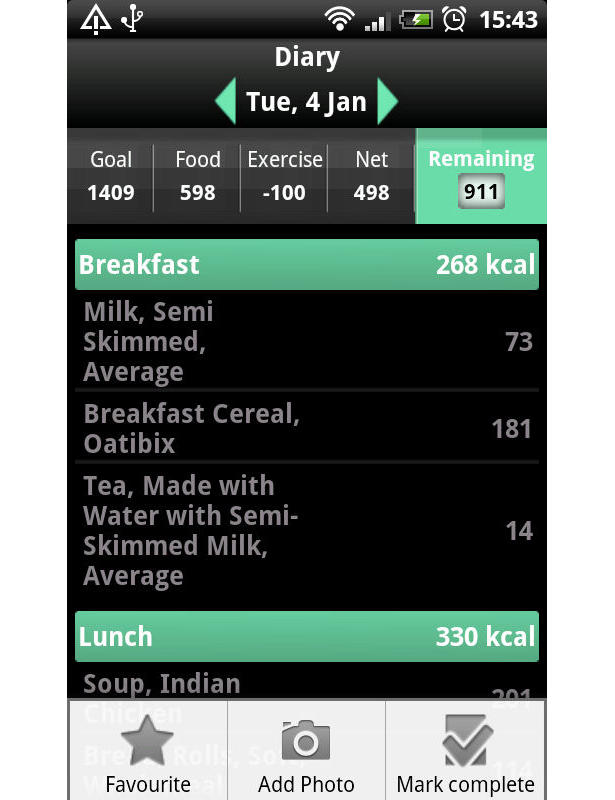
\includegraphics{Bilder/MMM.jpg}}
	\subfloat{	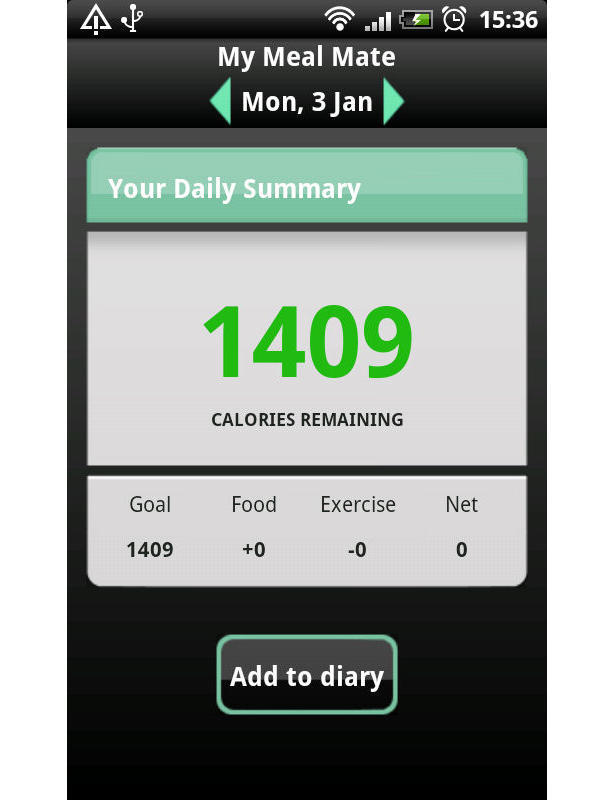
\includegraphics{Bilder/MMM2.jpg}}
	\caption[Screenshot der MMM Homepage]{Screenshot der MMM Homepage. Quelle: Carter et al., 2013}
	\label{bild2}
\end{figure}

%Abb 2: Screenshot der MMM Homepage. Quelle: Carter et al., 2013

Die App verfügt über eine Anbindung an ein Webinterface, in welches die gespeicherten Daten hochgeladen werden können. Treten Probleme beim Benutzen von MMM auf, haben Nutzer die Möglichkeit, sich die Funktionen der Applikation anhand zahlreicher verknüpfter Videos detailliert erklären zu lassen (Carter et al., 2013).



\subsubsection{Automated Self-Administered 24-hour Recall (ASA24)}

Basierend auf dem traditionellen 24-Stunden Protokoll wurde eine Methode entwickelt, die die Erfassung der Ernährung durch eine webbasierte Applikation verbessern soll. Das automatisierte 24-Stunden Protokoll wurde speziell entwickelt, um die Durchführbarkeit hochqualitativer Ernährungserhebung großer Gruppen zu verbessern. ASA24 ist ein kostenloses Instrument, welches online zur Verfügung steht. Es ist eine Weiterentwicklung der US Department of Agriculture Automated Multiple Pass Method (AMPM), die Interviewkomponente des NHANES (National Health and Nutrition Examination Survey). Diese wurde bereits bei Erhebungen mit großer Stichprobenzahl, wie dem nationalen Ernährungssurvey „What we eat in Amerika“, angewandt (Moshfegh et al., 2008).  ASA24, ein automatisiertes, selbstverwaltendes 24-Stunden Protokoll basiert auf zwei Internetseiten - einer Teilnehmerseite und einer Seite für  Wissenschaftler, welche die Verwaltung der Datensammlungen erlaubt und Zugang zu Analyse-Dateien gewährt. Die Teilnehmer können auf der für sie eingerichteten Internetseite ein Ernährungsprotokoll ausfüllen. Dabei werden sie mittels dynamischer Bedienungsmaske wie z.B. Animationen, visuellen und auditiven Hinweisen, durch das Programm geleitet. Die Nutzer werden gebeten, detaillierte Fragen zu Nahrungs- und Getränkeaufnahme sowie Verzehrzeiten zu beantworten. Weiterhin haben sie optional die Möglichkeit anzugeben, wo die Mahlzeiten eingenommen wurden, ob alleine oder in einer Gruppe gegessen wurde und ob sie währenddessen den Fernseher oder Computer genutzt haben. Die aufgenommenen Lebensmittel können in einer Suchfunktion aus einer Liste ausgewählt werden. Weitere Fragen zu Zubereitung und Portionsgrößen sind zu beantworten. Um die Portionsgrößen leichter einschätzen zu können, werden Fotos zum Vergleich herangezogen. Des Weiteren können Nahrungsergänzungsmittel angegeben werden. In Tabelle 2 ist der genaue Befragungsleitfaden aufgezeigt, nach welchem die Methode vorgeht. 

%TO DO:

%Tab. 6: Reihenfolge und Inhalt des ASA24 Ernährungsinterview-Leitfaden (Quelle: Subar et al., 2012)

\begin{table}[!h]
\begin{flushleft}
\caption{ Reihenfolge und Inhalt des ASA24 Ernährungsinterview-Leitfaden}
\end{flushleft}
\begin{tabular}{l p{8cm}}
ASA24 Leitfaden & Beschreibung der gesammelten Informationen \\
\hline\\

Mahlzeitenbasierte Kurzliste (MBK) &
Nutzer werden gebeten, Speisen, Uhrzeit und optional Ort, Computer/TV Nutzung und ob alleine oder in Gemeinschaft gegessen wurde, anzugeben. \\

Befragung zu Zwischenmahlzeiten &
Nutzer werden gefragt, ob sie in der Zeit zwischen den Mahlzeiten Speisen oder Getränke verzehrt haben.  Diese werden in die MBK eingetragen.\\

Details &
Nutzer werden gebeten, einzelne Details (z.B.  Form, Zubereitungsmethode, Portionsgröße, Zusätze) der in der MBK angegebenen Lebensmittel aufzulisten. \\

Vergessene Lebensmittel &
Nutzer werden zu häufig vergessenen Speisen und Getränken befragt, welche dann in die MBK eingetragen werden.\\

Letzte Überprüfung &
Nutzer werden gebeten, alle aufgelisteten Lebensmittel zu überprüfen und gegebenenfalls zu ergänzen.\\

Letzte Chance &
Nutzer haben nochmals die Möglichkeit, Lebensmittel zu ergänzen.\\

Üblicher Verzehr &
Nutzer werden gefragt, ob der gestrige Verzehr im Vergleich zum alltäglichen Verzehr mehr als üblich, üblich oder weniger als üblich war.\\


\end{tabular}
%\label{tab:ASA24}
\\Quelle: Modifiziert nach Subar et al.2012
\end{table}





\subsubsection{SenseCam}

Die SenseCam ist eine kleine mit Sensoren ausgestattete Kamera, die um den Hals getragen wird  und automatisch Fotos aus dem Blickwinkel des Nutzers schießt. Sie wurde entwickelt, um eine digitale Aufzeichnung vom Tag des Kameraträgers zu machen. Gesteuert durch äußere Einflüsse wie Bewegung, Wärme und Licht löst die Kamera alle 20 bis 30 Sekunden aus und speichert die Bilder auf einer integrierten Karte. Das Grundprinzip der SenseCam ist, dass nachdem eine digitale Aufzeichnung eines Ereignisses erfasst wurde, der Nutzer die Bilder anschließend anschauen kann, um seine Erinnerung aufzufrischen (Hodges et al., 2006). Solche tragbaren Kameras bieten viele Verwendungsmöglichkeiten. Eingesetzt werden sie zum Beispiel, um Menschen mit Gedächtnisstörungen als Erinnerungsstütze zu dienen (Browne et al., 2011). Weiterhin helfen sie als Ergänzung bei Ernährungserhebungen. Anhand der gespeicherten Fotos dokumentieren Nutzer und Ernährungswissenschaftler gemeinsam die am Vortag verzehrten Lebensmittel anhand des computergestützten 24-Stunden-Protokolls AMPM (Moshfegh et al., 2008).

\subsubsection{Remote Food Photography Method (RFPM)}

Die Remote Food  Photography Method, zu Deutsch „Ferngesteuerte Lebensmittel-Fotografie-Methode“, ist eine  Weiterentwicklung der Digital Photography of Foods Method (DPFM). In einer Studie, in der die Vergleichbarkeit der digitalen Fotografie und visueller Schätzverfahren zur Beurteilung der Nahrungsaufnahme überprüft wurde, zeigte sich die DPFM als neuartige und valide Methode, um den Lebensmittelverzehr in Cafeterien zu quantifizieren. Jedoch erwies sie sich als  unangemessen für alltägliche Lebensbedingungen (Williamson et al., 2003). Die RFPM wurde daraufhin speziell entwickelt, um die Ernährung im Alltag zu erheben. Dabei sollen die Nutzer in ihrem üblichen Essverhalten nicht eingeschränkt und die Portionsgrößen möglichst genau erfasst werden. Die Nutzer benötigen ein mit einer Kamera- und Datentransferfunktion ausgestattetes Mobiltelefon. Die zum Verzehr bestimmten Lebensmittel, ein Referenzmuster zur besseren Portionsgrößenabschätzung sowie eventuell entstehende Reste werden fotografiert und die Bilder mittels kabellosen Netzwerks zur Energie- und Nährstoffanalyse an einen Server verschickt. Um zu vermeiden, dass die Nutzer die Anwendung der RFPM vergessen, erhalten sie automatisch versendete Erinnerungen per Email und Textmittteilungen.  
Ein Fotoarchiv von über 2100 Standardportionsgrößen ermöglicht es Wissenschaftlern, eingesendete Fotos von Speisen entsprechenden Bildern aus dem Archiv zuzuordnen (Martin et al., 2009).




\subsubsection{EButton}

Der EButton ist ein kleiner Computer in Form eines Knopfes, der auf Brusthöhe getragen wird. Die integrierten Kameras schießen automatisch Fotos und speichern diese auf einer internen Speicherkarte. Anschließend werden die Fotos auf einen Computer übertragen. Der EButton nutzt die gleichen elektronischen Komponenten wie Smartphones. Es enthält einen leistungsfähigen Prozessor und viele Sensoren zur Datensammlung. Neben der Erfassung körperlicher Aktivität und der Hilfestellung für ältere und blinde Menschen, bietet der Minicomputer die Möglichkeit, objektive Informationen über den Verzehr der Nutzer zu erhalten.
Ohne dass der Nutzer die Kameras aktiv bedient, werden automatisch Fotos der auf dem Tisch platzierten Lebensmittel festgehalten. Wie in Abb. 4 zu sehen, umfassen die zwei integrierten  Weitwinkelkameras ein großes Sichtfeld für die Aufnahme der Speisen. Die Kameras schießen bei einer voreingestellten Geschwindigkeit, beispielsweise alle zwei Sekunden, ein Foto und speichern diese. Somit wird der gesamte Verzehr dokumentiert. Die Portionsgrößenberechnung erfolgt ebenfalls automatisch mittels einer speziell entwickelten Software. Einer großen Lebensmitteldatenbank werden anschließend Informationen über genaue Energie- und Nährstoffangaben entnommen (Sun et al., 2014). 

%TODO: FOTO EBUTTON EINFÜGEN
%Abb. 3: Reichweite der EButton-Kamera. Quelle: Sun et al. 2014

\begin{figure}[h]
	\centering
	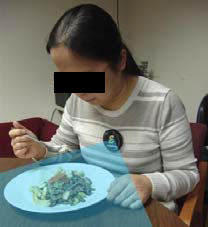
\includegraphics{Bilder/EButton.png}
	\caption[Reichweite der EButton-Kamera]{Reichweite der EButton-Kamera. Quelle: Sun et al. 2014}
	\label{bild3}
\end{figure}


\subsubsection{Mobile Telephone Food Record (mdFR)}

Bei der mdFR Methode fotografieren die Nutzer Speisen vor dem Essen und nach beendetem Verzehr. Die Energie- und Nährstoffaufnahme wird anhand automatischer Einteilung der Fotos, Identifizierung sowie Klassifizierung der Lebensmittel, Portionsgrößenberechnung und anschließender Nährstoffberechnung bestimmt. Benutzer sind in der Lage, falsch gekennzeichnete Lebensmittel oder Volumenberechnungen vor der Nährstoffberechnung manuell zu korrigieren (Zhu et al., 2010). Um ein geeignetes Bild  zu erhalten, müssen alle Nahrungsmittel und Getränke sowie ein Referenz-Marker im Foto enthalten sein. Die Einbeziehung eines Objekts bekannter Ausmaße ermöglicht das genauere Abschätzen des Volumens. Die gelungenen Bilder werden an einen Server gesendet, welcher die Fotos automatisiert analysiert. Der Nutzer erhält eine Rückmeldung über die ermittelten Lebensmittel und bestätigt, bzw. korrigiert diese. Durch Verknüpfung zu einer Nährstoffdatenbank werden  Energie- und Nährstoffaufnahme anhand der Informationen aus Bildanalyse und Volumenschätzung berechnet. Die Ergebnisse können dann Ernährungswissenschaftlern übergeben werden (Six et al., 2010).

%TODO: BILD mdFR EINFÜGEN 
%Abb. 3: Prozess der Portionsgrößenberechnung
%Quelle: Modifiziert von Zhu et al., 2010

\begin{figure}[h]
	\centering
	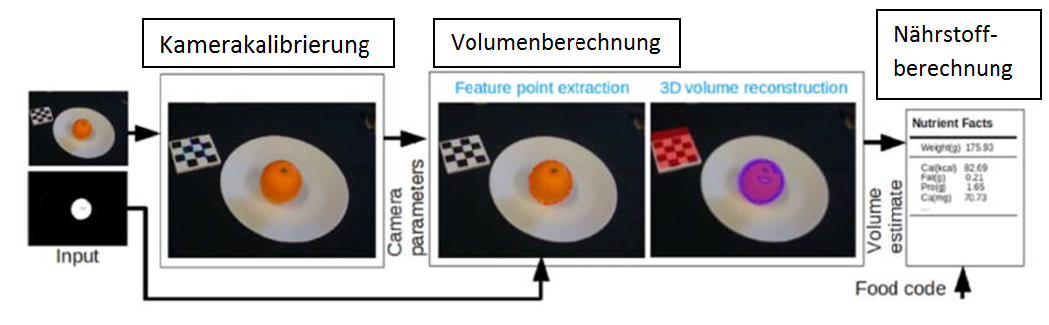
\includegraphics[width=0.9\textwidth]{Bilder/mdFR.png}
	\caption[Prozess der Portionsgrößenberechnung]{ Prozess der Portionsgrößenberechnung. \\ Quelle: Modifiziert von Zhu et al., 2010}
	\label{bild4}
\end{figure}


%--------------------------------------- LITERATURANALYSE ------------------------------------------------------------------------------------


\newpage
\section{Literaturanalyse}

Im folgenden Kapitel wird jeweils eine Studie pro in Kapitel 2.3 vorgestellter  computergestützter Ernährungserhebungsmethode vorgestellt, anhand derer die Validität der Methode aufgezeigt werden soll.  Zunächst wird die Auswahl der Studien kurz erläutert. Daraufhin werden die einzelnen Studien samt Methodik und Ergebnis beschrieben. 

\subsection{Erläuterung der Auswahl}

Die Auswahl der Studien basiert auf den Ergebnissen der Datenbanken Pub Med, ACM Digital Library und IEEE eXplore, welche Datenbanken für  Forschungsliteratur zu computergestützten Ernährungserhebungsmethoden darstellen. Gesucht wurde anhand der Stichpunkte ''Nutrition'', ''Mobile'', ''Telephone'', ''Dietary Assessment'', ''Elderly'', ''Smartphone'', ''Computer'', ''Adolescents'' und Kombinationen daraus. Ergebnisse, welche die eingegebenen Stichworte in einem anderen Kontext behandelten, wurden herausgefiltert. Der zeitliche Rahmen umfasst die Jahre 2010 bis 2014. Es wurde aus den geeigneten Studien jeweils eine Studie zu jeder Methode ausgewählt, welche diese getestet und beurteilt hat. Ergebnisse weiterer Studien werden in den Diskussionsteil der Arbeit einfließen, da eine detaillierte Beschreibung aller einflussnehmenden Studien über den Rahmen dieser Arbeit hinausgehen würde. Eine Übersicht über die sechs Studien und deren Charakteristika ist in Kapitel 4 zu finden. Die einzelnen Studien werden in diesem Kapitel beschrieben.

Nach Sharp und Allman-Farinelli (2014) können die vorgestellten Methoden in folgende drei Kategorien unterteilt werden:
\begin{itemize}
\item Erhebungsmethoden, die Ernährung durch Computerprogramme erfassen
\item Erhebungsmethoden, die Ernährung mittels Fotographie und manueller Analyse erfassen
\item Erhebungsmethoden, die Ernährung automatisiert erfassen
\end{itemize}

Die Studien zu My Meal Mate, Remote Food Photography Method und Mobile Device Food Record werden entsprechend von Sharp und Allman-Farinelli in diese Kategorien einsortiert. Die verbleibenden drei Studien lassen sich eindeutig in die entsprechenden Kategorien einordnen. Alle Studien sind in den entsprechenden Kategorien in Tabelle 7 aufgeführt. 

%TODO: TABELLE GESAMTÜBERSICHT EINFÜGEN

%Tab.7: Gesamtübersicht über die Zuordnung der Studien zu den Hauptkategorien

\begin{table}[!h]
\begin{flushleft}
\caption{Gesamtübersicht über die Zuordnung der Studien zu den Hauptkategorien}
\end{flushleft}
\begin{tabular}{p{6cm} p{8cm}}
Hauptkategorien & Ausgewählte Studien \\
\hline\\

Erhebungsmethoden, die Ernährung durch Computerprogramme erfassen &
\textbf{Carter et al. (2012)}: "My Meal Mate": validation of the diet measures captured on a smartphone application to facilitate weight loss \\
&
\textbf{Kirkpatrick et al. (2014)}: Performance of the Automated Self-Administered 24-hour Recall relative to a measure of true intakes and to an interviewer-administered 24-h recall \\

Erhebungsmethoden, die Ernährung mittels Fotographie und manueller Analyse erfassen &
\textbf{Gemming et al. (2013)}: Feasibility of a SenseCam-assisted 24-h recall to reduce under-reporting of energy intake \\
&
\textbf{Martin et al. (2012)}: Validity of the RFPM for estimating energy and nutrient intake in near real-time \\

Erhebungsmethoden, die Ernährung automatisiert erfassen &
\textbf{Lee et al. (2012)}: Comparison of Known Food Weights with Image-Based Portion-Size Automated Estimation and Adolescents’ Self-Reported Portion Size \\
&
\textbf{Jia et al. (2013)}: Accuracy of food portion size estimation from digital pictures acquired by a chest-worn camera 


\end{tabular}
%\label{tab:Überblick}
\end{table}
\newpage

%------------------------------------- Erhebung durch Computerprogramme -----------------------------------------------------------------------

\subsection{Studien zu Erhebungsmethoden, die Ernährung durch Computerprogramme erfassen}

\textbf{1) "My Meal Mate" (MMM): validation of the diet measures captured on a smartphone application to facilitate weight loss (Carter et al. 2012)}\\
Das Ziel der Validitätsstudie war herauszufinden, ob MMM Potential zu einer erfolgreichen Ernährungserhebungsmethode hat. Als Referenzmethode diente ein am Telefon durchgeführtes 24-Stunden Protokoll.

\textbf{Methodik}\\
Teilnehmer der Studie waren 50 Mitarbeiter und Studenten der Universität Leeds. In einer Schulung erlernten  die Freiwilligen den Umgang mit dem Smartphone und der App. Anschließend erfassten die Freiwilligen über einen Zeitraum von sieben aufeinanderfolgenden Tagen ihre Ernährung mit „My Meal Mate“. Es stand ihnen frei, ob sie die Erhebung verteilt über den Tag oder am Abend durchführen. Wenn sie den Verzehr des Tages am Abend durchführen wollten, sollten sie Fotos von den Mahlzeiten als Erinnerungshilfe machen. Waren sich die Teilnehmer bzgl. der Portionsgrößen unsicher oder die in der Applikation vorgegebenen Größen schienen unpassend, durften sie die Speisen wiegen und das entsprechende Gewicht eingeben. Innerhalb des Erhebungszeitraums wurde außerdem zweimal unangekündigt ein telefonisches 24-Stunden Erinnerungsprotokoll durchgeführt. Dabei war es wichtig, dass die Teilnehmer während der Befragung nicht die in die App eingetragenen Daten als Erinnerungsstütze nutzen. Die Energie- und Nährstoffaufnahmen der Erhebungstage wurden mit den erfassten Daten der Protokolle der jeweiligen Tage verglichen.
Die Analyse erfolgte mittels statistischer Software und verschiedener statistischer Tests, wie dem gepaarten t-Test, um Energie- und Nährstoffaufnahmen der Methoden zu vergleichen.

\textbf{Ergebnis}\\
Da nicht alle Teilnehmer die Erhebung beendet haben, konnten nur 320 von 350 Einträgen (94\%) bewertet werden.  
Am ersten der zwei Tage, an dem  sowohl MMM als auch das Telefoninterview durchgeführt wurde, konnte kein signifikanter Unterschied  zwischen den Methoden bei der Energie- und Nährstoffaufnahme aufgezeigt werden (gepaarter t-Test). Der Unterschied lag bei 16kcal (68kJ). Am zweiten Tag konnte ein signifikanter Unterschied von 105kcal (441kJ) festgestellt werden. Die 24-Stunden Befragung erfasste durchschnittlich eine höhere Aufnahme als MMM. Die Korrelation zwischen MMM und dem 24-Stunden Protokoll für die Energie- und Nährstoffaufnahme erwies sich als moderat bis hoch und statistisch signifikant  (Korrelationskoeffizient).\\


\textbf{2) Performance of the Automated Self-Administered 24-hour Recall relative to a measure of true intakes and to an interviewer-administered 24-h recall (Kirkpatrick et al. 2014)}\\
Ziel der Studie war es, ASA24 mittels einer Verzehrsstudie zu validieren. Dabei wurde die bei drei Mahlzeiten aufgenommene Essensmenge vor und nach dem Verzehr genau bestimmt. Das Interviewgestützte 24-Stunden Erinnerungsprotokoll fungierte als Referenzmethode.

\textbf{Methodik}\\
Die Studie umfasste eine Teilnehmerzahl von 83 Personen zwischen 20 und 70 Jahren. Die ausgewählten Teilnehmer nahmen am ersten Tag der Studie drei Mahlzeiten (Frühstück, Mittagessen und Abendessen) im Studienzentrum ein. Die Speisen und Getränke wählten sie von einem Buffet. Alle ausgewählten Lebensmittel wurden unauffällig vor und nach dem Verzehr gewogen, um die tatsächlich aufgenommene Menge jedes Teilnehmers zu bestimmen. In Speisesälen installierte Kameras filmten die Teilnehmer während des Verzehrs, um eventuell extern mitgebrachte Speisen und ein Teilen der Lebensmittel untereinander zu dokumentieren. Es gab keine Beschränkungen bei der Aufnahme mitgebrachter Speisen und Getränke, jedoch wurden diese von der Analyse ausgeschlossen. Weiterhin wussten die Teilnehmer nicht, dass sie am folgenden Tag ein 24-Stunden Erinnerungsprotokoll ausfüllen werden sollten. \\
Am zweiten Tag wurden die Studienteilnehmer zufällig in zwei Gruppen aufgeteilt. Eine Hälfte füllte den ASA24 Fragebogen an Computern aus, die andere Hälfte durchlief die von Interviewern am Telefon durchgeführte 24-Stunden-Befragung (AMPM). Bei beiden Methoden protokollierten die Teilnehmer den Verzehr des Vortages von Mitternacht bis Mitternacht. Wissenschaftler erstellten und überprüften eine Liste aller genannten Lebensmittel. Diese half ihnen zu bestimmen, ob die genannten Lebensmittel mit den angebotenen Speisen übereinstimmen. Übereinstimmungen  wurden eingeteilt in „exakt“, „nah“ und „fern“. Eine exakte Übereinstimmung war zum Beispiel die Angabe eines fettarmen Joghurts, eine nahe Übereinstimmung ein Joghurt mit regulärem Fettgehalt, wenn im Rahmen der Studie ein fettarmer Joghurt angeboten wurde.  Nach Beendigung der Ernährungserhebungen führten die Teilnehmer als letzten Schritt eine computergestützte Befragung zu Demographie und Gesundheitsverhalten durch. 
Die Auswertung erfolgte mittels verschiedener statistischer Tests. Zum Beispiel wurden lineare Regressionsmodelle verwendet, um zu beurteilen, ob die Unterschiede zwischen tatsächlicher und berichteter Aufnahme signifikant sind.

\textbf{Ergebnis}\\
Von 83 Teilnehmern beendeten 40 den ASA24 und 41 den AMPM. Teilnehmer der ASA24 Befragung gaben zu 80% die verzehrten Lebensmittel richtig an („exakte“, „nahe“ und „ferne“ Übereinstimmungen zusammengefasst). Beim AMPM waren es 83\%. Demnach war kein signifikanter Unterschied   (lineare Regressionsmodelle) feststellbar. 
Die Anzahl vergessener Angaben unterschied sich insgesamt kaum zwischen beiden Methoden. Sowohl bei ASA24 (36,1\%) als auch bei AMPM (29,1\%) wurden Zugaben und Zutaten zu Lebensmitteln bei Speisen und Getränken, die aus mehreren Komponenten bestehen, häufiger vergessen als bei Speisen und Getränken mit wenigen Komponenten. 
Bei ASA24 konnten signifikante Unterschiede   (lineare Regressionsmodelle) zwischen tatsächlichem und angegebenem Verzehr bei Berechnungen zur Fett- und Vitamin-D Aufnahme und gefunden werden. Dabei war die protokollierte Fettaufnahme geringer als der tatsächlich verzehrte und die Vitamin-D Aufnahme höher. Bei der 24-Stunden Befragung ergaben sich signifikante Unterschiede bei mehreren Komponenten, z.B. Kohlenhydrate, Salz, Gemüse und Zucker. Die angegebene Menge lag jeweils höher als die tatsächlich zugeführte. 


%------------------------------- Fotografie und manuell -----------------------------------------------------------------------------------------

\subsection{Studien zu Erhebungsmethoden, die Ernährung mittels Fotographie und manueller Analyse erfassen}
Zwei der ausgewählten computergestützten Methoden lassen sich zu Erhebungsverfahren zusammenfassen, welche die Ernährung mittels Fotographie und manueller Analyse durch Ernährungswissenschaftler erheben. Studien zum SenseCam gestützten 24-Stunden Protokoll und zur RFPM sind im Folgenden beschrieben.

\textbf{3) Feasibility of a SenseCam-assisted 24-h recall to reduce under-reporting of energy intake (Gemming et al. 2013)}

Tragbare Kameras wie die SenseCam könnten die 24-Stunden Befragung verbessern. Ziel der Studie war es zu beurteilen, ob die SenseCam als Unterstützung für das 24-Stunden Erinnerungsprotokoll geeignet ist. Es galt herauszufinden, zu welchem Grad die Fotos die Angaben der Befragten unterstützen und verändern. Im Einzelnen hatte die Studie das Ziel, die Wirkung der Fotos auf die vom Teilnehmer gemachten Energie- und Nährstoffangaben zu erfassen.

\textbf{Methodik}\\
Die Teilnehmerzahl umfasste 13 gesunde Erwachsene zwischen 18 und 65 Jahren aus England. Die Teilnehmer trugen die SenseCam über einen Zeitraum von zwei Tagen. Am dritten Tag führten sie zunächst ein Interview-gestütztes 24-Stunden Erinnerungsprotokoll durch, basierend auf der AMPM Befragung.  Nach beendeter Erhebung wurden die mit der SenseCam aufgenommenen Fotos herangezogen. Die Teilnehmer konnten das Protokoll daraufhin mit Lebensmitteln ergänzen, welche sie ohne Bilder als Erinnerungsstütze vergessen hatten. Zusätzlich füllten die Teilnehmer einen Fragebogen zur persönlichen Einschätzung der SenseCam aus. Abschließend folgte ein Vergleich zwischen Energie- und Nährstoffaufnahmen der beiden Methoden sowie die Auswertung der Fragebögen.

\textbf{Ergebnis}\\
Daten von zehn Teilnehmern wurden analysiert. Das Einbeziehen der Bilder erhöhte die angegebene Energieaufnahme um rund 1432 $\pm$ 1564 kJ oder 12,5\% im Vergleich zum AMPM 24-Stunden Erinnerungsprotokoll. Der Anstieg war vor allem auf die Angabe von 41 zusätzlichen Lebensmitteln (17\%) zurückzuführen. Es gab insgesamt acht Änderungen von Portionsgrößen, davon waren fünf Volumenerhöhungen. Die Auswirkung auf die Gesamtenergiezufuhr war jedoch gering (-259 bis 189kJ). Fehlerhafte Angaben, wie zum Beispiel Lachs anstatt Hühnchen, hatten dabei größere Effekte auf die Energiezufuhr (-787 bis 165kJ), als fehlerhafte Angaben zu Obst und Gemüse. 
Die Teilnehmer empfanden die Fotos als Erinnerungsstütze hilfreich und konnten so genauere Angaben über die verzehrten Lebensmittel machen. Das Tragen der SenseCam zur Ernährungserfassung empfanden die meisten Teilnehmer als gering belastend. Drei Nutzer gaben an, dass sie das Tragen der Kamera in der Öffentlichkeit manchmal als unangenehm empfanden. Nach eigenen Angaben beeinflusste die SenseCam nie (50\%), selten (10\%) oder manchmal (40\%) die Essgewohnheiten. Fünf Teilnehmer gaben an, dass sie höchstens eine Woche lang die SenseCam einsetzen würden, vier Teilnehmer zwei bis drei Tage und ein Teilnehmer einen Monat lang. \\


\textbf{4) Validity of the RFPM for estimating energy and nutrient intake in near real-time (Martin et al. 2012)}\\
Die Studie verfolgte vier Ziele. Zunächst wurde die Validität der Methode bei der Schätzung der Energieaufnahme im Vergleich zur DLW Methode getestet. Zweitens wurde die Zuverlässigkeit der Methode bei der Schätzung von Energie- und Nährstoffzufuhr während zwei Mahlzeiten beurteilt. Drittens wurde untersucht, ob durch RFPM ein verändertes Essverhalten (Over- oder Undereating) zu beobachten ist. Als letztes wurden die Teilnehmer anhand eines Fragebogens nach ihrer Zufriedenheit mit der Methode befragt.

\textbf{Methodik}\\
Es nahmen 50 Erwachsene zwischen 18 und 65 Jahren an der Studie teil. Fast 90\% der Teilnehmer waren übergewichtig oder adipös (BMI $\geq$ 25). Die Probanden nutzten RFPM zur Ernährungserhebung während zwei Mittagsmahlzeiten. Sie konnten sich individuell aus einer Reihe vorgegebener Lebensmittel Speisen zusammenstellen. Die Portionsgrößen der verzehrten Lebensmittel wurden vor und nach der Nahrungsaufnahme gewogen, um beide Ergebnisse vergleichen zu können. Anschließend wurde über einen Zeitraum von zwei Wochen die Energie- und Nährstoffaufnahme über die DLW Methode bestimmt. Währenddessen verwendeten die Teilnehmer RFPM zur Bestimmung von Energie- und Nährstoffaufnahme im alltäglichen Leben über einen Zeitraum von einer Woche. Die Ergebnisse der DLW Methode und der RFPM wurden miteinander verglichen. Die Zufriedenheit der Teilnehmer mit der Erhebungsmethode wurde mittels einer Skala von 1 bis 6 bewertet. Dabei stand 6 für die höchste Zufriedenheit.

\textbf{Ergebnis}\\
Die Daten von 49 Teilnehmern der zwei Mittagsmahlzeiten wurden analysiert. Die Ergebnisse der zwei Methoden unterschieden sich nicht signifikant. Die durch RFPM berechneten Daten zur Energie- und Nährstoffaufnahme lagen durchschnittlich nur 4 $\pm$ 73 kcal oder 1,2 $\pm$ 15,1\% unter der durch Abwiegen erlangten Ergebnisse. 
Zur Auswertung der DLW Methode sowie der einwöchigen Ernährungserhebung mit RFPM wurden Werte von 42 Probanden durchleuchtet. Die mit RFPM gemessene Energieaufnahme unterschied sich nicht signifikant   Intraclass-Korrelation und Bland-Altman Analyse zu der mit DLW bestimmten Aufnahme. Die RFPM unterschätzte die Energieaufnahme um 152 $\pm$ 694 kcal/Tag oder 3,7\%. 
In der Woche, in der die RFPM genutzt wurde, um die Ernährung zu erfassen, konnte kein signifikantes  Over- oder Undereating festgestellt werden. 
Auf einer Skala von 1 bis 6 bewertete die Mehrheit der Teilnehmer (82\%) ihre allgemeine Zufriedenheit mit der RFPM mit 5 oder höher. Die Benutzerfreundlichkeit der Methode bewerteten 93\% der Probanden mit 5 oder höher. 


%------------------------------ Automatische Erfassung ------------------------------------------------------------------------------------------

\subsection{Studien zu Erhebungsmethoden, die Ernährung automatisiert erfassen}


\textbf{5) Comparison of Known Food Weights with Image-Based Portion-Size Automated Estimation and Adolescents’ Self-Reported Portion Size (Lee et al. 2012)}\\
Die Ziele der Studie waren es (1) die Fehlerquote der automatisch berechneten Portionsgrößen im Vergleich zu bekannten Portionsgrößen zu bestimmen und (2) die Fehler von automatischer Berechnung und dem Schätzen der Portionsgrößen durch die Jugendlichen selbst zu vergleichen.

\textbf{Methodik}\\
Es wurden willkürlich 15 gesunde Jugendliche zwischen elf und 18 Jahren für die Studie ausgewählt. Im Umfang der Studie nahmen die Teilnehmer alle Mahlzeiten innerhalb von 24 Stunden unter Beobachtung zu sich. Bei jeder Mahlzeit erfassten sie anhand von Smartphones Fotos der Lebensmittel vor und nach dem Verzehr. Auf den Bildern mussten alle Speisen und Getränke sowie ein Referenzmuster abgebildet sein. Die gelungenen Fotos wurden zur automatischen Energie- und Nährstoffanalyse an einen Server gesendet. Die Jugendlichen schätzten zudem anhand der Fotos die Portionsgrößen für das Frühstück. Dafür verwendeten sie zwei verschiedene Methoden, welche sich jeweils unterschiedlicher Hilfsmittel bedienen. 
Schließlich wurden die Werte bekannter, automatisch berechneter und geschätzter Portionsgrößen miteinander verglichen.

\textbf{Ergebnis}\\
Portionsgrößen für insgesamt 19 verschiedene Lebensmittel wurden bestimmt. Die tatsächliche Energieaufnahme der Teilnehmer lag durchschnittlich bei 2723 $\pm$ 51 kcal. Die automatische Berechnung der Energieaufnahme (EA) ergab mit 3588 $\pm$ 180 kcal einen größeren Wert. Von den 19 Lebensmitteln fallen durch automatische Bestimmung rund 50\% der Portionsgrößen in einen akzeptablen Bereich. Zum Beispiel wichen automatisch berechnete Volumen von Lebensmitteln wie Würstchen, Erdbeermarmelade und Cheeseburger nur zu höchstens 15\% von den tatsächlichen Portionsgrößen ab. Einige Berechnungen wichen dagegen stark vom eigentlichen Gewicht ab. Das Volumen von Salat beispielsweise wurde zu 400\% überschätzt. Verglichen zu den Portionsgrößenschätzungen der Jugendlichen zeigt die automatische Berechnung bessere Ergebnisse. Zwar konnten die Teilnehmer wenige Portionsgrößen der verzehrten Lebensmittel gut abschätzen, jedoch wichen die Volumen der automatischen Berechnung im Durchschnitt deutlich geringer von den tatsächlichen Volumen der Nahrungsmittel ab. \\


\textbf{6) Accuracy of food portion size estimation from digital pictures acquired by a chest-worn camera (Jia et al. 2013)}

Genaue Schätzung der Portionsgrößen ist bei der Ernährungserhebung von großer Bedeutung. Von den EButton-Bildern können die entsprechenden Portionsgrößen der abgebildeten Lebensmittel halbautomatisch mit Hilfe einer Computersoftware berechnet werden. Das Ziel der Studie war es, die Genauigkeit der aus den mit EButton geschlossenen Fotos berechneten Portionsgrößen zu bewerten. Als Referenz dienten zum einen Volumenschätzungen und zum anderen eine genaue Berechnung der Portionsgrößen mittels physikalischer Messung.

\textbf{Methodik}\\
Sieben Labormitarbeiter trugen den EButton einmalig während des Mittagessens an sieben verschiedenen Orten der Forschungsstätte (z.B. Kantine oder Büro). Das exakte Volumen der einzelnen Lebensmittel wurde zunächst mittels physikalischer Messung bestimmt. Danach nahmen die Studienteilnehmer die Speisen zu sich, während die im EButton integrierte Kamera Fotos der Lebensmittel aufnahm. Nach Beendeter Mahlzeit identifizierte eine Software die Lebensmittel automatisch und berechnete die einzelnen Volumen. Zur weiteren Überprüfung der Genauigkeit der Software, wurden drei Bewertungspersonen einberufen, die das Volumen der einzelnen Lebensmittelproben durch die Betrachtung der selben Bilder schätzten.

\textbf{Ergebnis}\\
Insgesamt wurden Fotos von 100 Lebensmitteln gesammelt und die Volumen berechnet. Durchschnittlich lag der Unterschied zwischen der berechneten Portionsgröße und dem tatsächlichen Volumen aller Proben bei -2,8\% mit einer Standardabweichung von 20,4\%. Bei 85 Proben unterschieden sich die Ergebnisse aus der Softwareberechnung und der tatsächlichen physikalischen Messung nicht mehr als 30\%. Bei einem Vergleich der Volumenschätzungen zwischen Software und Bewertungspersonen zeigte die Softwareberechnung viel weniger Bias und Variabilität.

\newpage

\begin{landscape}
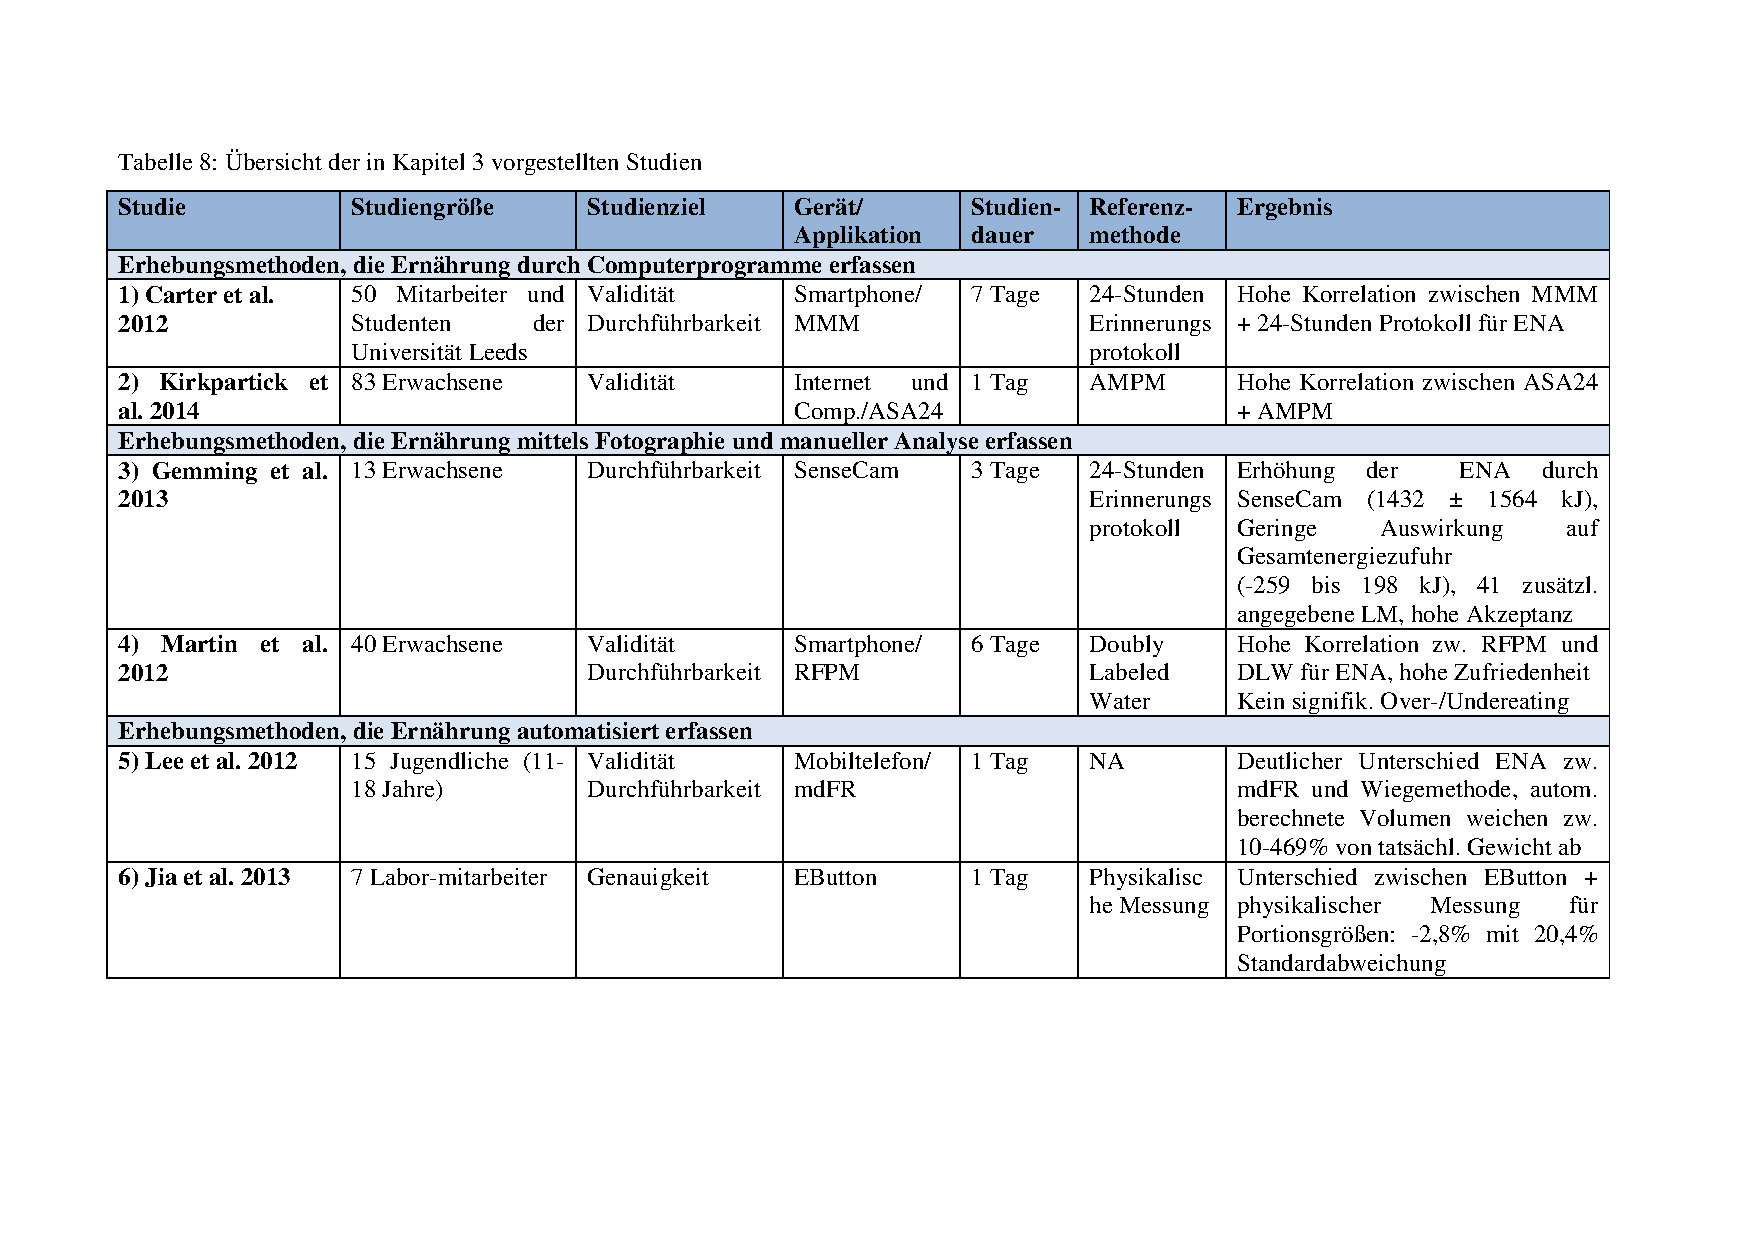
\includepdf[fitpaper]{Bilder/Tabelle8.pdf}
\end{landscape}

\nocite{*}


% ----------------------------------------------------------------------------------------------------------
% Kapitel
% ----------------------------------------------------------------------------------------------------------
\section{Diskussion}

\subsection{Vor- und Nachteile traditionieller direkter Ernährungserhebungsmethoden}


\subsection{Vor- und Nachteile computergestützter Ernährungserhebungsmethoden}

- Der Teilnehmer erfasst seinen Verzehr sofort und kann so keine Angaben vergessen 
\subsection{Vergleich von üblichen und computergestützten Methoden}



\section{Schlussbetrachtung/Ausblick}


% ----------------------------------------------------------------------------------------------------------
% Literatur
% ----------------------------------------------------------------------------------------------------------
\renewcommand\refname{Literaturverzeichnis}
\printbibliography
%\bibliographystyle{myalpha}
\pagebreak

% ----------------------------------------------------------------------------------------------------------
% Anhang
% ----------------------------------------------------------------------------------------------------------
\pagenumbering{Roman}
\setcounter{page}{1}
\lhead{Anhang \thesection}

\begin{appendix}
%\section*{Anhang}
\phantomsection
%\addcontentsline{toc}{section}{Anhang}
\addtocontents{toc}{\vspace{-0.5em}}

%\section{GUI}
%Ein toller Anhang.

%\subsection*{Screenshot}
%\label{app:screenshot}
%Unterkategorie, die nicht im Inhaltsverzeichnis auftaucht.

\end{appendix}


\newpage
\thispagestyle{empty}
\begin{center}
	\vspace*{5em}
	\huge\textbf{Erklärung}\\
\end{center}
\vspace{2em}
Ich versichere persönlich, dass ich die vorstehende Arbeit selbständig und ohne Benutzung anderer als der angegebenen Hilfsmittel angefertigt habe. Alle Stellen, die wörtlich oder sinngemäß aus Veröffentlichungen entnommen sind, wurden als solche kenntlich gemacht. Die Arbeit ist in gleicher oder ähnlicher Form oder auszugsweise im Rahmen einer anderen Prüfung noch nicht vorgelegt worden.

\vspace{2em}
\begin{minipage}{\linewidth}
	\begin{tabular}{p{15em}p{15em}}
	Bonn, den 27.10.2014
	\end{tabular}
\end{minipage}




\end{document}
